\documentclass[DIV=20]{scrartcl}

\usepackage{amsmath}
\usepackage{systeme}
\usepackage{listings}
\usepackage{graphicx}



\begin{document}

\begin{titlepage}
	\centering
	\vspace{3cm}
	{\itshape\Large CONTROL AVANZADO DE PROCESOS INDUSTRIALES, SISTEMAS NAVALES Y AEROESPACIALES	 \par}
	% {\bfseries\LARGE Universidad Superior T\'ecnica \par}
	\vspace{3cm}
	{\scshape\Huge Control de sistema caótico \par}
	\vfill
	{\Large Fernando Ayats Llamas \par}
	{\Large 15 de Febrero 2023 \par}
\end{titlepage}

\section{Sistema}

El sistema que se controla en este trabajo es un sistema hipercaótico. Un
sistema caótico es aquel que para ciertas condiciones iniciales $X_A$ y $X_B$,
aunque sean muy cercanas, las trayectorias que sigan con el desarollo del
sistema inevitablemente divergirán, hasta que sean irreconocibles.
Por otra parte, el sistema es de dimensión 5, por lo que la dinámica que
presenta es más compleja de lo normal. Por eso usamos el prefijo \emph{hiper}.

Las ecucaciones del sistema en tiempo discreto se describen a continuación,
junto con una representación de las dos primeras componentes de una simulación
que se ha dejado ejecutar durante unos segundos.


\begin{align*}
	 & x_{(n, k+1)} = x_{(n, k)} + g_n  dt                   \\
	 & g_1 = a_1 x_1 - a_2 x_2 + a_3 x_3 + a_4 x_4 - a_1 x_5 \\
	 & g_2 = a_5 x_1 - a_6 \arctan{a_7 x_2} + u_2            \\
	 & g_3 = - a_8 x_1 - a_4 x_4 + u_3                       \\
	 & g_4 = a_9 x_3 - a_{11} x_5 + u_4                      \\
	 & g_5 = a_{10} x _4 + u_5                               \\
\end{align*}

Los parámetros para el sistema de estudio:

\begin{align*}
	 & a_1 = 0.6    \\
	 & a_2 = 10.0   \\
	 & a_3 = 1.5    \\
	 & a_4 = 1.5    \\
	 & a_5 = 0.5    \\
	 & a_6 = 3.8    \\
	 & a_7 = 28.0   \\
	 & a_8 = 0.2    \\
	 & a_9 = 0.19   \\
	 & a_{10} = 0.9 \\
	 & a_{11} = 0.6 \\
\end{align*}

\begin{figure}[h]
	\centering
	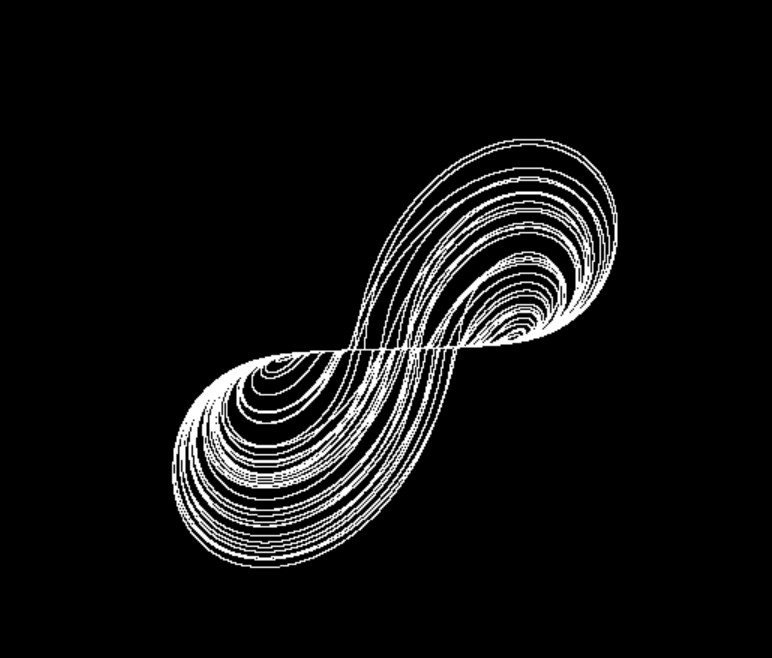
\includegraphics[width=8cm]{caos}
\end{figure}

\section{Control}

El sistema será controlado con una señal $u$ impulsiva, como se ha expuesto en
las ecuaciones del sistema. La señal de control se aplica según una superficie
de control tal que el $signo(x_2)$ cambie. Cuando esto suceda, se aplica las
ecuaciones de control, que se desarrollan el programa del trabajo en la sección siguiente.

\section{Programación}

Para la simulación del sistema, se ha utilizado un programa en Basic del que se
incluye el siguiente código:

\lstinputlisting[basicstyle=\tiny]{main.bas}

\section{Resultados}

Los resultados de la simulación muestran un control del sistema, que se mantiene
en una trayectoria estable durante un periodo de convergencia. A continuación se
muestra una representación de esta trayectoria:

\begin{figure}[h]
	\centering
	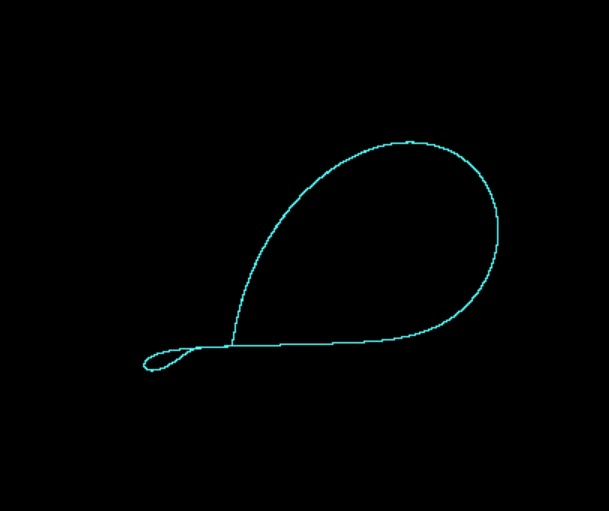
\includegraphics[width=8cm]{control}
\end{figure}

\end{document}
